\section{Force estimation}
In order to have a representation of the reaction force on the Endowrist, we must resort to estimation.
Because of the reasons mentioned in section II, the force cannot be measured using sensors and thus have to rely on mathematical models as functions of torque measurements.

\subsection{Mathematical model}
The main challenge we face in making a model lies in the fact that the pulley system on the Endowrist is non-linear, and thus its full dynamics cannot be modeled in a simple manner. In other words, to have an accurate representation of force we require a higher order model.
Regardless, a physical linear model for grip force can be derived \cite{kim2014dynamic}.
A clear representation of grip force is important to the operator because it helps prevent excess grip application to soft tissue.
This serves as a good starting point for a useable dynamical model.

\begin{figure}
\centering
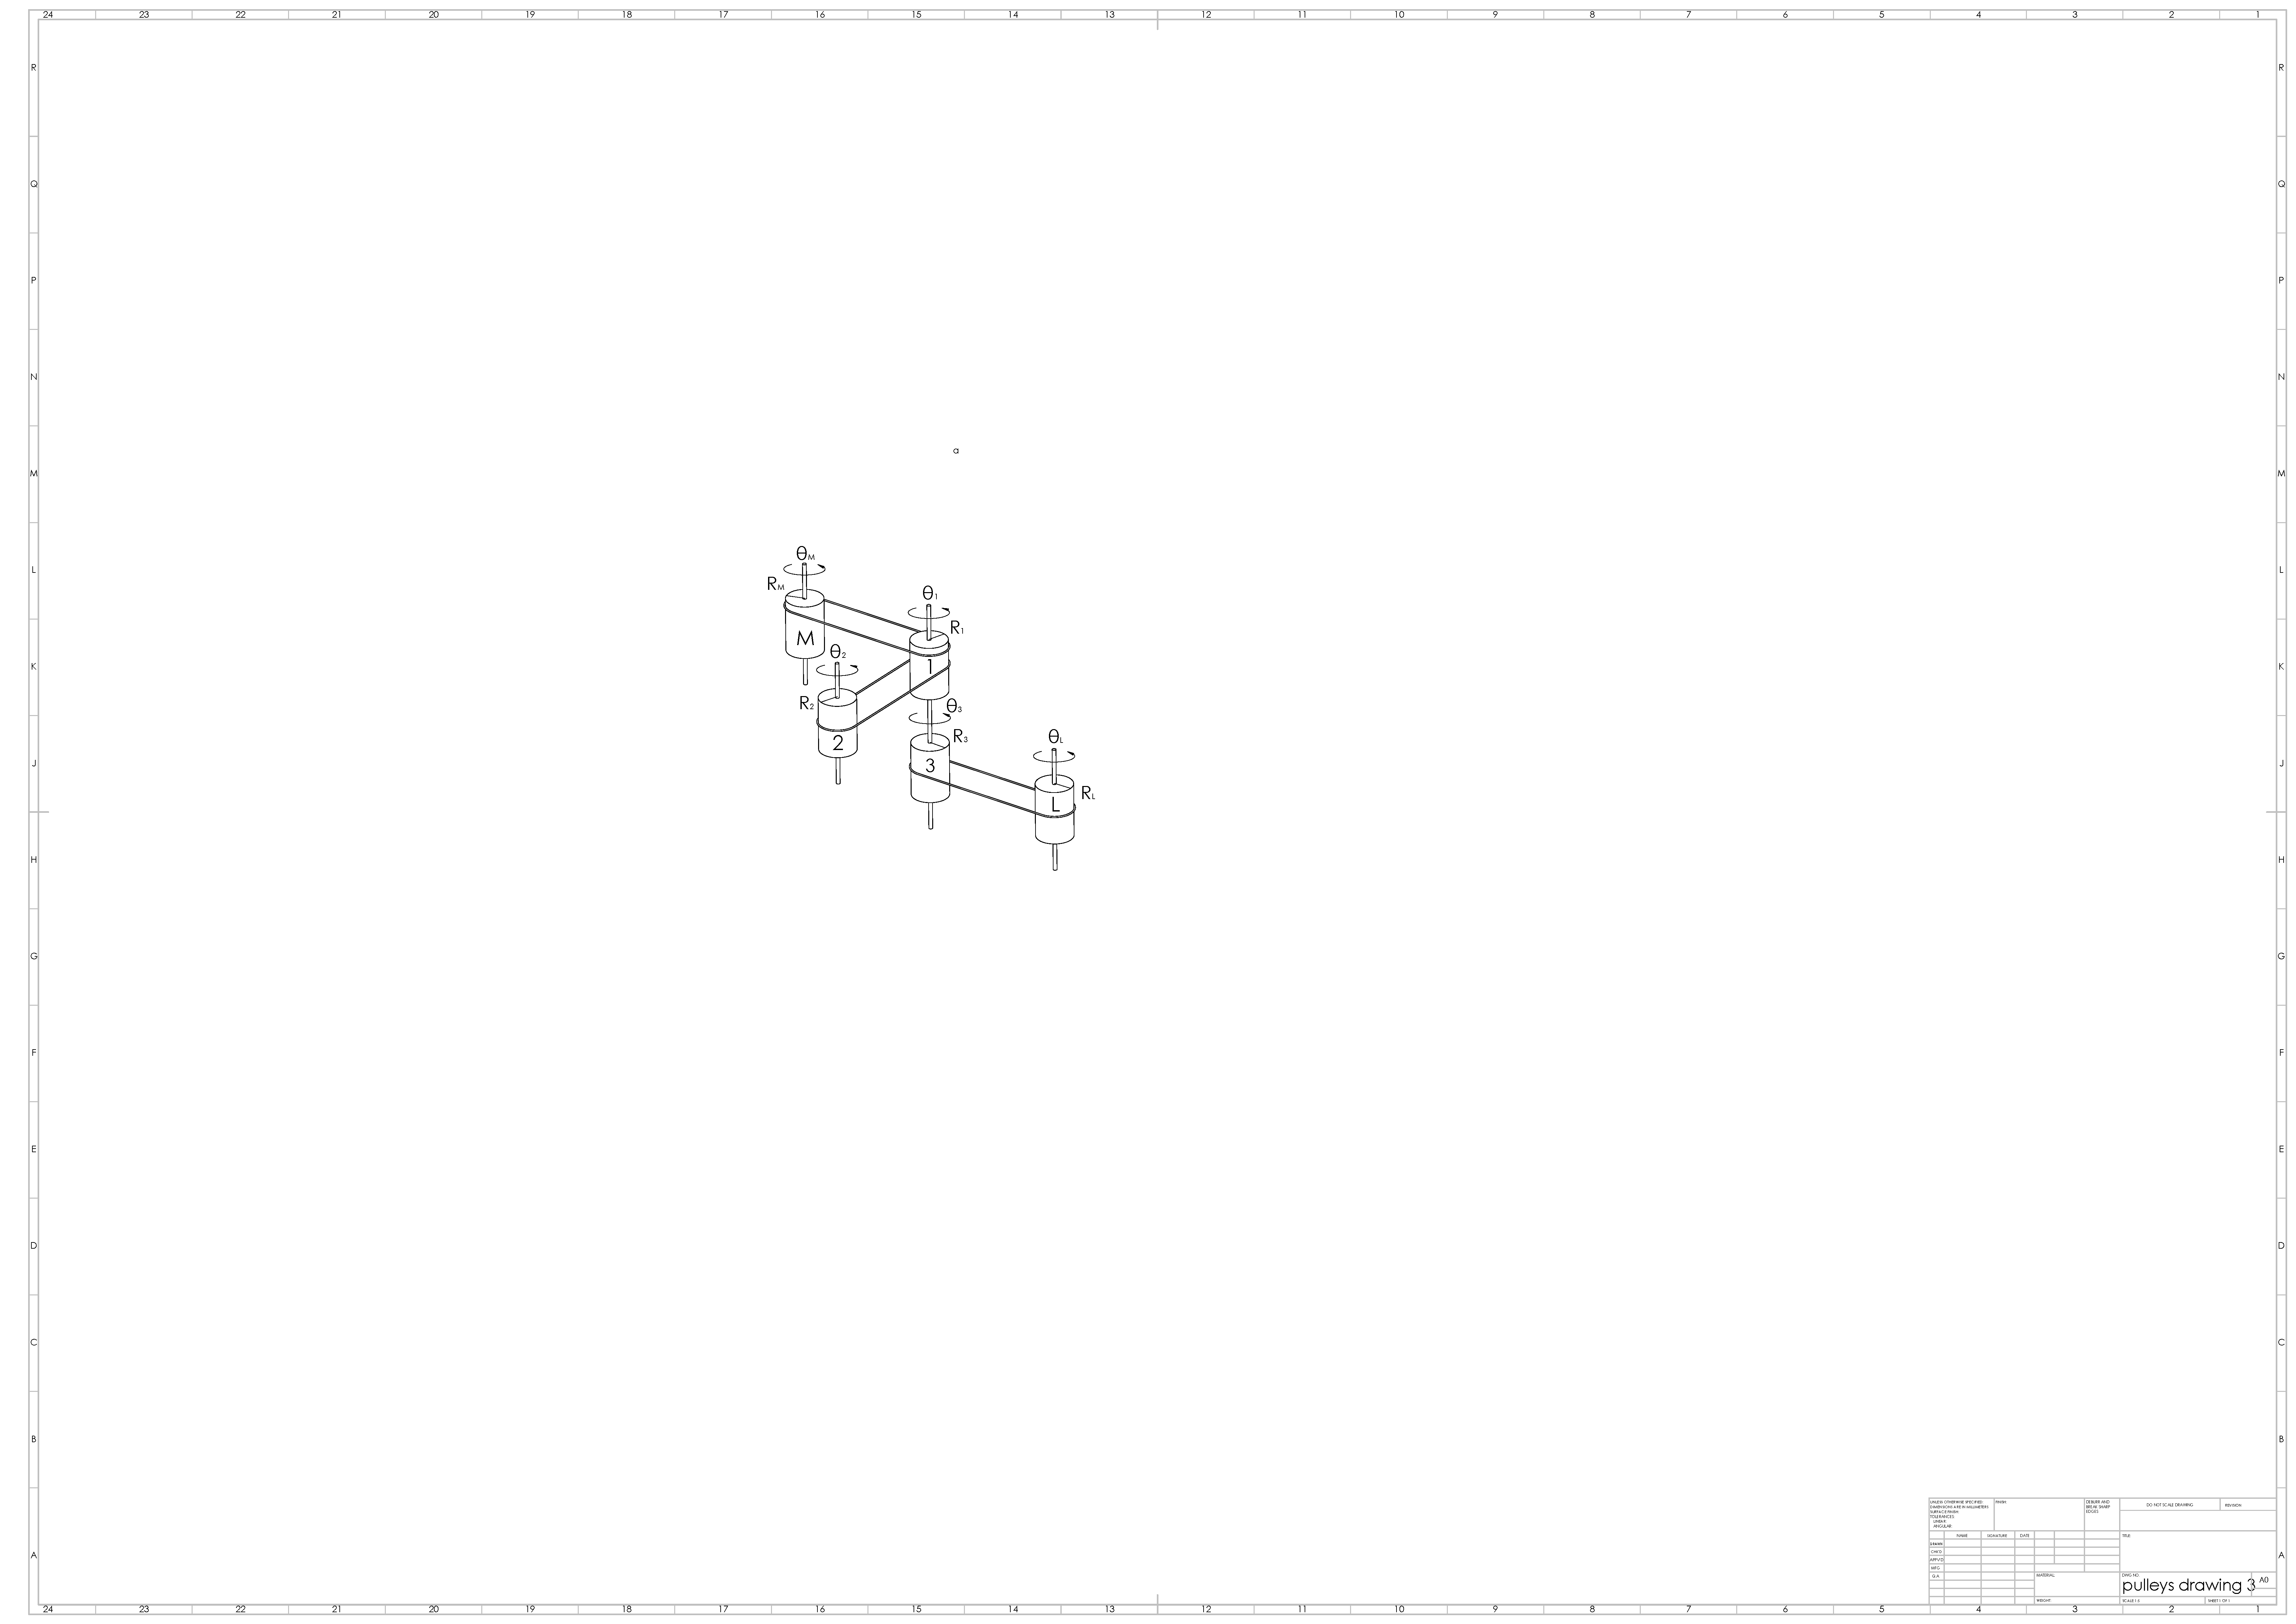
\includegraphics[width=\linewidth]{pulleys.pdf}
\caption{The pulley system of the Endowrist gripper modeled in \cite{kim2014dynamic}.}
\end{figure}

The dynamical model in \cite{kim2014dynamic} is simplified to a 10th order state space system with 31 abstract, non-physical parameters (\ref{sspace}-10).
This is done to simplify the process of parameter estimation.

% ATTENTION !!
% Before each equal sign include a & like this &=
% it will make the equal signs stand in a line!!
%\begin{gather}
%\begin{align}
%J_m\ddot{{\theta}_m} + B_m \dot{{\theta}_m} + R_m T_{m1}(R_m {\theta}_m - R_1 {\theta}_1) &= u_m\\
%J_L\ddot{{\theta}_L} + B_L \dot{{\theta}_L} + R_L T_{L3}(R_L {\theta}_L - R_3 {\theta}_3) &= u_L
%\end{align}
%\end{gather}

\begin{gather}\label{sspace}
\begin{align} 
\dot{x_1} &= x_2\\
\dot{x_2} &= A_1x_1 + A_2x_2 + A_3x_3 + A_5x_5 + A_7x_7\\
\dot{x_3} &= x_4\\
\dot{x_4} &= B_1x_1 + B_3x_3 + B_4x_4 + B_5x_5 + B_FF\\
\dot{x_5} &= x_6\\
\dot{x_6} &= C_1x_1 + C_3x_3 + C_5x_5 + C_6x_6 + C_9x_9\\
\dot{x_7} &= x_8\\
\dot{x_8} &= K_mu_m + M_1x_1 + M_7x_7 + M_8x_8\\
\dot{x_9} &= x_{10}\\
\dot{x_{10}} &= K_Lu_L + L_5x_5 + L_9x_9 + L_{10}x_{10}
\end{align}
\end{gather}

In equations (\ref{sspace}-10), $x_i$ represents the i-th state space vector element, while $u_L$ and $u_m$ represent the input signals for the pulley motors. 
The state vector is described in (\ref{statevector}).
\begin{align} \label{statevector}
\mathbf{x} &= 
\begin{bmatrix}
\theta_1 &\dot{\theta_1} &\theta_2 &\dot{\theta_2} &\theta_3 &\dot{\theta_3} &\theta_m &\dot{\theta_m} &\theta_L &\dot{\theta_L} \\
\end{bmatrix}^T
\end{align}

Additionaly, we can model the outwards force output by the yaw mechanism.
This is done by simple measurment with the setup in figures \ref{fig:entire_force_testsetup} and \ref{fig:endeffector_force}.

% \begin{align}\label{eq:dyn_1}
% J_m\ddot{{\theta}_m} + B_m \dot{{\theta}_m} + R_m T_{m1}(R_m {\theta}_m - R_1 {\theta}_1) = u_m
% \end{align}
% \begin{align}\label{eq:dyn_2}
% J_L\ddot{{\theta}_L} + B_L \dot{{\theta}_L} + R_L T_{L3}(R_L {\theta}_L - R_3 {\theta}_3) = u_L
% \end{align}
% \begin{multline}\label{eq:dyn_3}
% J_1\ddot{{\theta}_1}+ B_1 \dot{{\theta}_1} + R_1 T_{12}(R_1{\theta_1} - R_1{\theta}_3 - R_2{\theta_2})\\ = R_1 T_m(R_m{\theta}_m - R_1{\theta}_1)
% \end{multline}
% \begin{align}\label{eq:dyn_4}
% J_2\ddot{{\theta}_2}+ B_2 \dot{{\theta}_2} + LF = R_2 T_{12}(R_1{\theta_1} - R_1{\theta}_3 - R_2{\theta_2})
% \end{align}
% \begin{multline}\label{eq:dyn_5}
% J_3\ddot{{\theta}_3}+ B_3 \dot{{\theta}_3} + R_1 T_{12}(R_1{\theta_1} - R_1{\theta}_3 - R_2{\theta_2})\\ = R_3 T_{L3}(R_L{\theta}_L - R_3{\theta}_3)
% \end{multline}

%\todo{we should include what each variable corresponds to (T, J, R, F, theta)} NOT ANYMORE

%From equations \ref{eq:dyn_1}-\ref{eq:dyn_5} it is visible that this system can be converted to a linear state space model.
%Moreover, simplifying the equations by replacing physical coefficients with general ones results in a 10th order state space model with 31 parameters.
%This is the model we will perform parameter identification on.


\subsection{Parameter identification}
Parameter identification is performed using the Matlab parameter identification toolbox.
For us to tune the model parameters, it is necessary for us to perform experiments for input-output measurement datasets.

We do this by applying a known torque to the Endowrist actuators and measuring the output force $F$.
The goal here is to get a fully parametrized state space model which we can then use for grip force estimation with a Kalman filter.

At the time of wiriting this article, we are stil in the process of developing a full setup for fitting the state space model for grip force.
On the other hand , the outwards force model can be approximated linearly in a piecewise manner.
This is done by using a linear approximation based on input torque and output downwards force measurement.

\begin{figure}
  \centering
  \begin{subfigure}{.45\linewidth}
    \centering
    \vspace{24pt}
    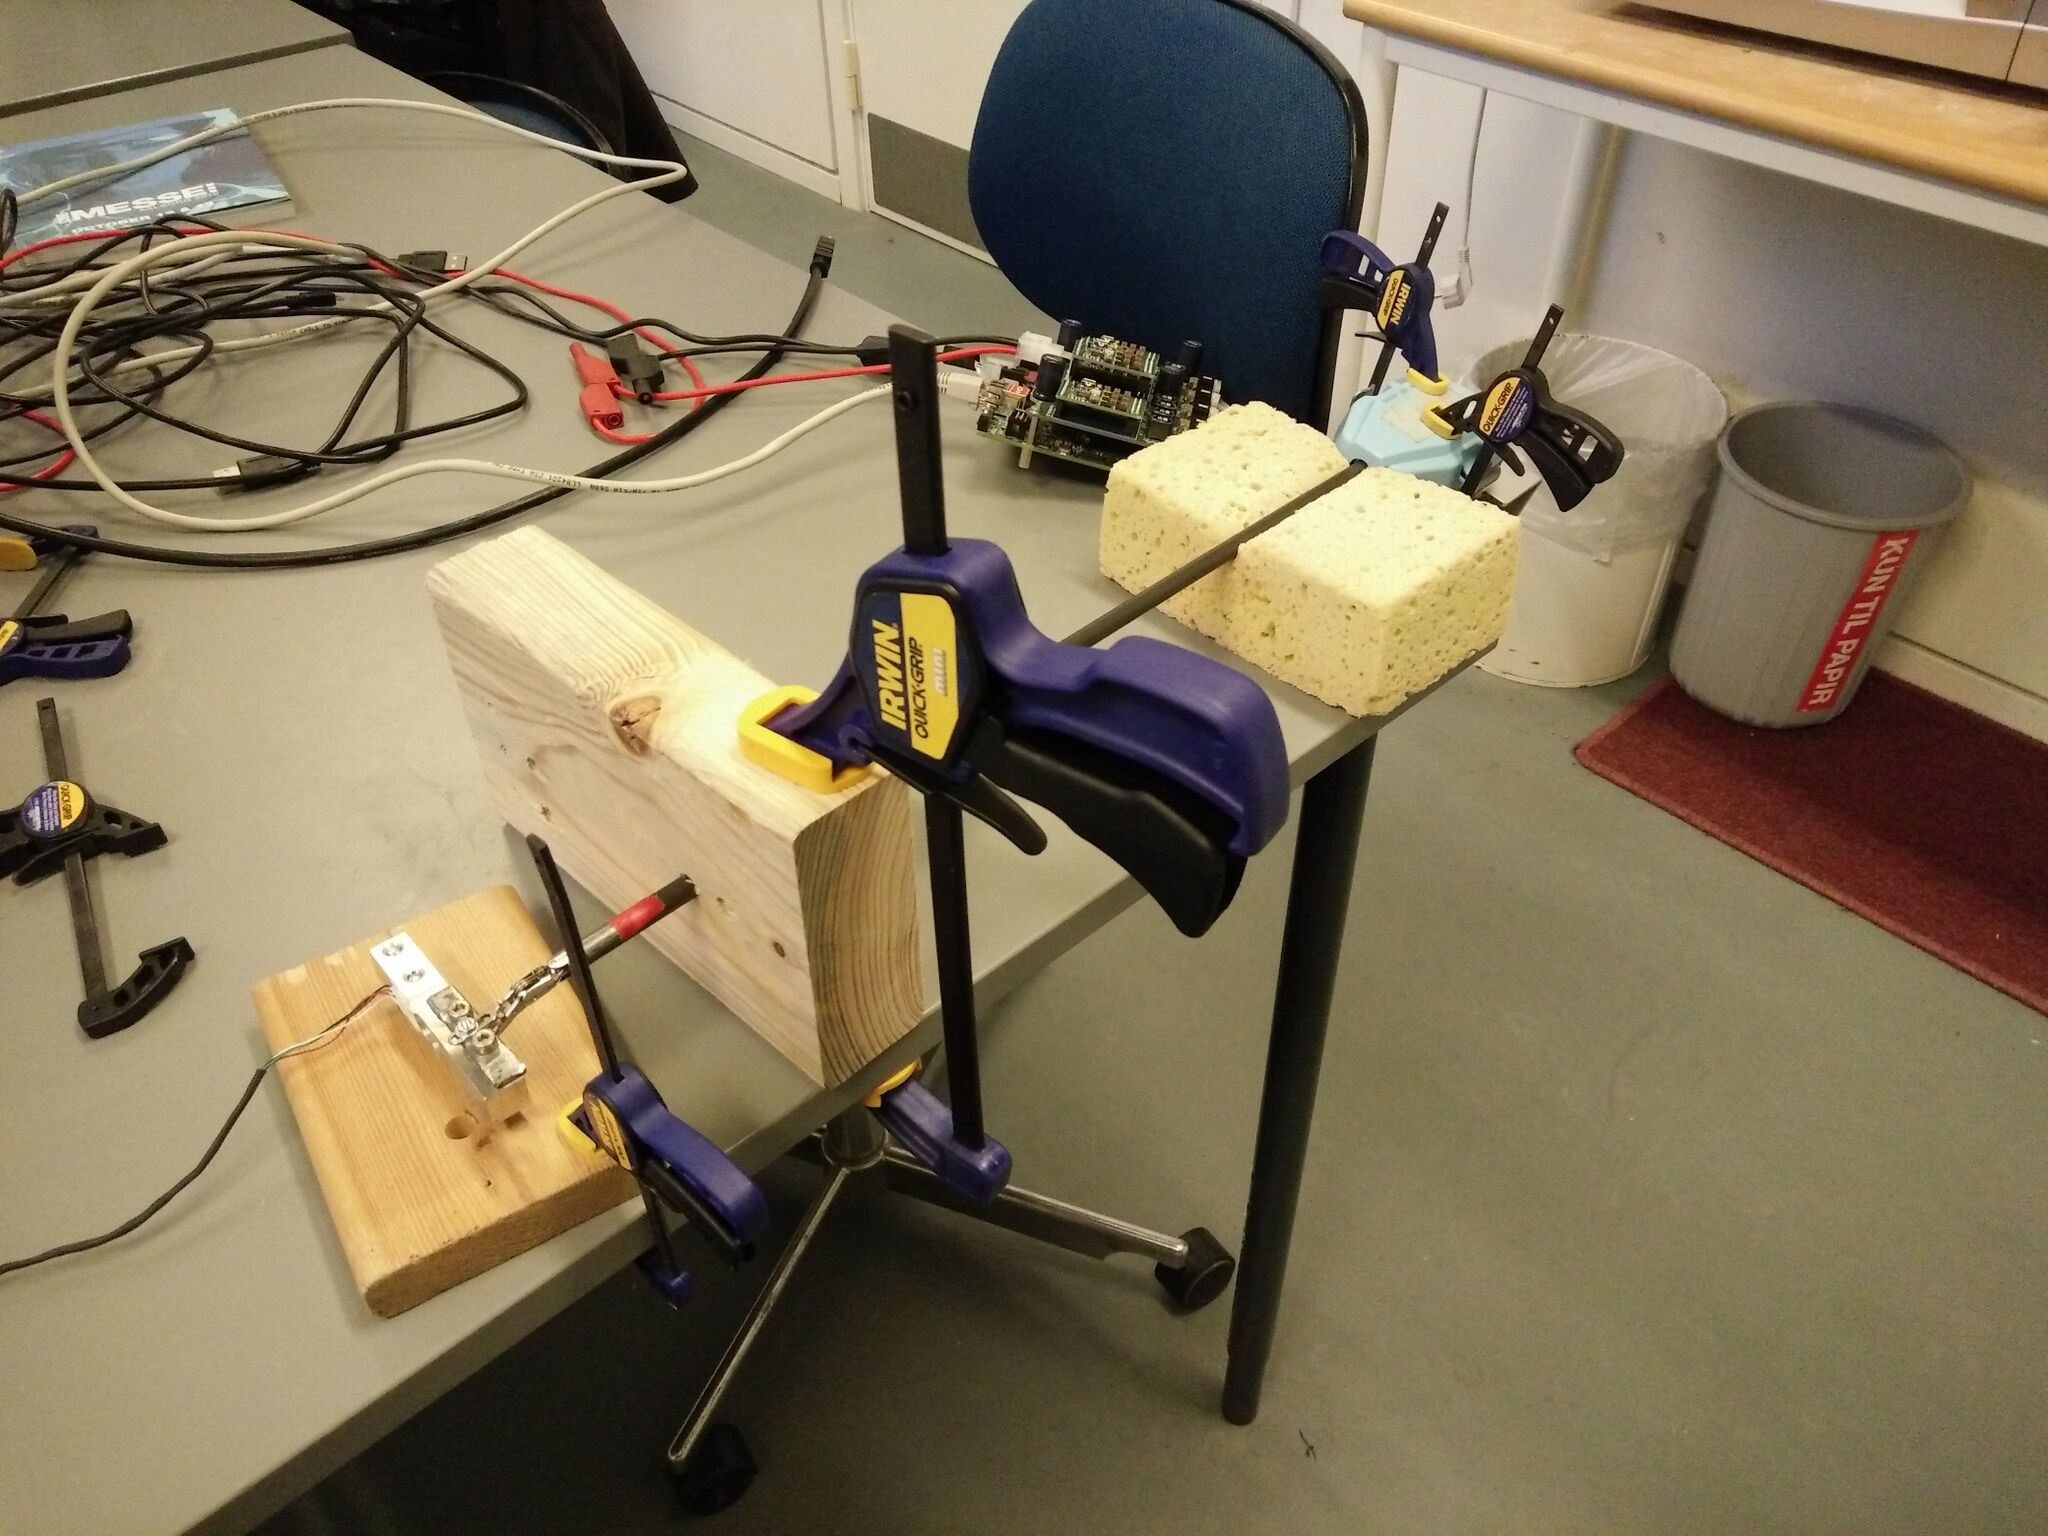
\includegraphics[width=\linewidth]{overall_force.jpg}
    \caption{The entire test setup. From the right, a scale for measuring the downwards force, a piece of wood for stiffening the Endowrist and keeping it it place and the Endowrist holder with motors.}
    \label{fig:entire_force_testsetup}
  \end{subfigure}
  \begin{subfigure}{.45\linewidth}
    \centering
    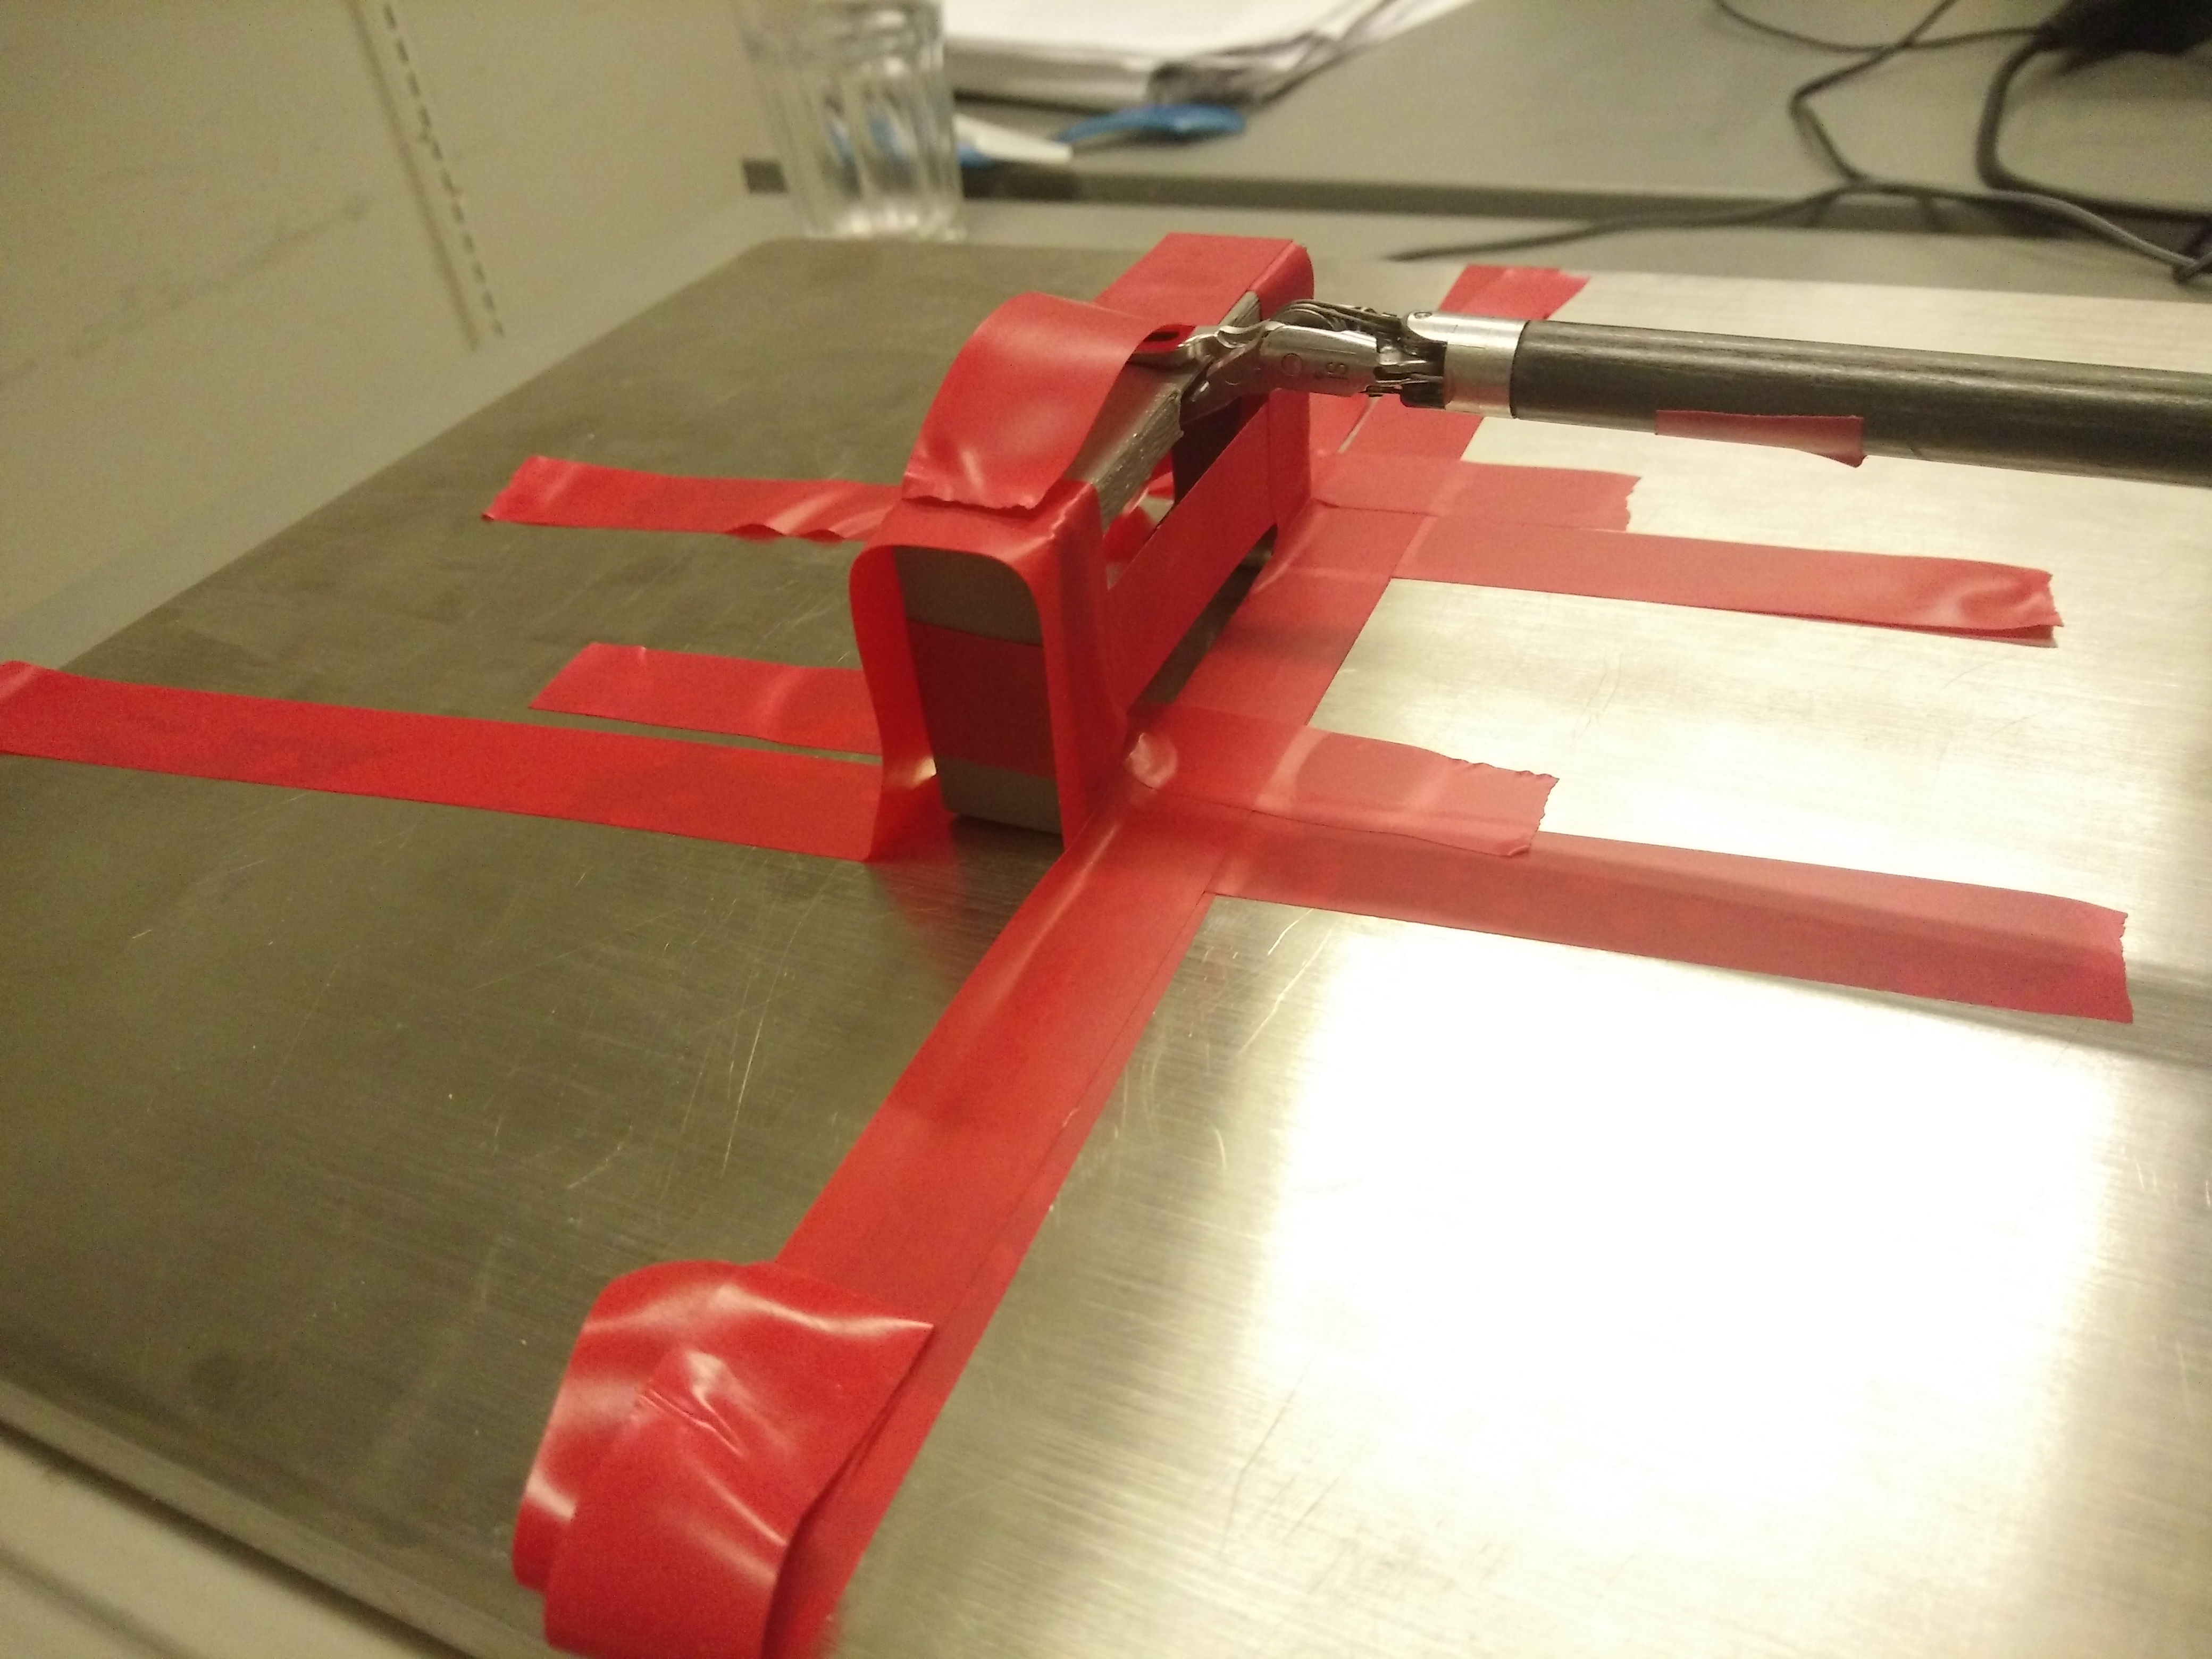
\includegraphics[width=\linewidth]{endeffector_force.jpg}
    \caption{A 3D printed case which made it possible to make an orthogonal force from the end-effector to the scale.}
    \label{fig:endeffector_force}
  \end{subfigure}
\caption{Test setup for the force estimation of the end-effector.}
\label{fig:Overview_force}
\end{figure}

A piecewise linear expression is made from the 340 mA sample and up and can be seen on \eqref{eq:linear_force_endo}.

\begin{equation}
\text{y} = 0.0028 \cdot \text{x} -0.8259 
\label{eq:linear_force_endo}
\end{equation} 

We consider the above equation appropriate for feedback loop implementation.